\documentclass[a4paper]{article}

\usepackage[UTF8]{ctex}
\usepackage[a4paper,margin=1in]{geometry}
\usepackage{graphicx}
\usepackage{float}
\usepackage{listings}
\usepackage{longtable}
\usepackage{booktabs}
\usepackage{hyperref}
\usepackage{fancyhdr}
\usepackage{lastpage}
\usepackage{color}
\usepackage{indentfirst}        % 首段缩进
\setlength{\parindent}{2em}     % 缩进2字符
\usepackage{zhnumber}           % 中文编号
\usepackage[dvipsnames]{xcolor}

%\newcommand{\college}{中山大学计算机学院}
\newcommand{\projname}{数据库系统原理实验|实验四}
\newcommand{\reporttitle}{数据库视图与控制实验}
\newcommand{\stuno}{23336179}
\newcommand{\authorname}{马福泉}
\newcommand{\major}{计算机科学与技术}
\newcommand{\adviser}{赖韩江}
\newcommand{\startdate}{2025年10月16日}
\newcommand{\labenddate}{2025年10月19日}
\newcommand{\labroom}{B202}

\pagestyle{fancy} % 使用 fancyhdr 风格
\fancyhf{}      % 清空默认的页眉页脚

% 设置页眉
\fancyhead[L]{\kaishu \projname}      % 左侧页眉显示项目名称
\fancyhead[C]{\kaishu \reporttitle}    % 中间页眉显示报告标题
\fancyhead[R]{\kaishu \authorname} % 右侧页眉显示作者姓名

% 设置页脚
\fancyfoot[C]{第 \thepage 页，共 \pageref{LastPage} 页} % 中间页脚显示页码

% 去除页眉页脚与正文之间的分隔线
\renewcommand{\headrulewidth}{0.4pt}
\renewcommand{\footrulewidth}{0pt}

% 设置文档背景颜色
\definecolor{mybgcolor}{RGB}{0, 0, 0} % 定义背景颜色
\definecolor{NavyBlue}{RGB}{0,0,128} % 添加颜色定义
% \pagecolor{mybgcolor} % 设置背景颜色

% listing 配置rust
% \lstdefinelanguage{Rust}{
%   keywords={fn, let, mut, struct, enum, impl, pub, use, mod, trait, where},
%   keywordstyle=\color{NavyBlue},
%   comment=[l]{//},
%   commentstyle=\color{gray},
% }
% \lstset{language=Rust}

\lstset{
  basicstyle=\ttfamily\small,
  keywordstyle=\color{NavyBlue},
  commentstyle=\color{gray},
  stringstyle=\color{red},
  showstringspaces=false,
  extendedchars=false, % 关键：不处理中文
  breaklines=true
}

\begin{document}

% 封面
\begin{titlepage}
    \centering
    
\includegraphics[width=10cm]{img/SYSULogo.png}

    \vspace{1em}
    %{\Large \college \par}
    \vspace{1em}
    {\Large \kaishu \projname \par}
    \vspace{3em}

    

    
    {\fontsize{40pt}{42pt}\kaishu \selectfont \boldmath \reporttitle\par}
    \vspace*{\fill}

    \begin{center}
    {\Large
    \makebox[5em][s]{学号}:\underline{\makebox[15em][c]{\kaishu \stuno}}\\[1em]
    \makebox[5em][s]{姓名}:\underline{\makebox[15em][c]{\kaishu \authorname}}\\[1em]
    \makebox[5em][s]{专业}:\underline{\makebox[15em][c]{\kaishu \major}}\\[1em]
    \makebox[5em][s]{课程教师}:\underline{\makebox[15em][c]{\kaishu \adviser}}\\[1em]
    \makebox[5em][s]{起始日期}:\underline{\makebox[15em][c]{\kaishu \startdate}}\\[1em]
    \makebox[5em][s]{结束日期}:\underline{\makebox[15em][c]{\kaishu \labenddate}}\\[1em]
    \makebox[5em][s]{实验地点}:\underline{\makebox[15em][c]{\kaishu \labroom}}
    }
    \end{center}

    \vspace*{\fill}
\end{titlepage}

% 目录
\tableofcontents
\newpage


\section{实验概述}

\subsection{实验目的}

熟悉使用SQL语言支持的有关视图的操作，能够熟练地使用SQL语句来创建需要的视图，对视图进行查询和取消等。

熟悉SQL的数据控制功能，能够使用SQL语句来向用户授予和收回权限。

\subsection{实验内容}

在实验二修改后的数据库基础上，进行视图操作和数据控制实验，要求附上执行结果（数据库）截图。

\subsubsection{视图操作}

1. 更新数据库，将数据库图书表的借阅次数(interviews\_times)修改如下：

\begin{table}[H]
\centering
\caption{更新后的图书表}
\label{tab:updated_books}
\begin{tabular}{|p{1.2cm}|p{2.5cm}|p{2.5cm}|p{2.5cm}|p{2.5cm}|p{1.5cm}|p{1.5cm}|}
\hline
\textbf{book\_id} & \textbf{book\_name} & \textbf{book\_isbn} & \textbf{book\_author} & \textbf{book\_publisher} & \textbf{interviews\_times} & \textbf{book\_price} \\
\hline
b0001 & SQL Server 2012宝典 & 978-7-121-22013-5 & 廖梦怡 & 电子工业出版社 & 38 & 89.00 \\
\hline
b0002 & 职称英语专用教材 & 978-7-121-14800-2 & 孙若红 & 电子工业出版社 & 15 & 45.00 \\
\hline
b0003 & 中国通史 & 978-7-5388-53155 & 于海娣 & 黑龙江科学技术出版社 & 60 & 68.00 \\
\hline
b0004 & 丰子恺儿童文学选集 & 978-7-5007-8972-7 & 丰子恺 & 中国少年儿童出版社 & 32 & 22.50 \\
\hline
b0005 & 英语同义词辨析词典 & 978-7-5135-2294-6 & 赵同水 & 外语教学与研究出版社 & 29 & 55.00 \\
\hline
b0006 & 数据库基础与应用 & 978-7-304-06430-3 & 徐孝凯 & 中央广播电视大学出版社 & 5 & 35.00 \\
\hline
b0007 & 微积分初步 & 978-7-304-03742-0 & 赵坚 & 中央广播电视大学出版社 & 48 & 17.00 \\
\hline
b0008 & ASP.NET从入门到精通 & 978-7-302-28753-7 & 明日科技 & 清华大学出版社 & 17 & 89.80 \\
\hline
\end{tabular}
\end{table}

2. 创建视图，用于查看借阅次数大于25次的图书信息。\\
3. 创建视图，用于查看借阅了图书的读者姓名，以及他们借阅的图书名称。\\
4. 创建视图，用于查询借阅次数大于35次的图书名称和借阅次数，并在视图中为列指定别名"BOOKNAME"和"TIMES"。\\
5. 创建视图, 使用With Check Option, 创建一个只包含中央广播电视大学出版社的图书视图，然后通过该视图分别增加、删除、修改一条出版社是中央广播电视大学出版社和清华大学出版社的图书记录，验证With Check Option是否起作用。\\
6. 上面的四个视图可更新吗？通过SQL更新语句分别进行验证。\\
7. 删除上面视图。

\subsubsection{数据控制}

创建三个用户USER1, USER2，USER3

1. 授予所有用户对图书表的查询权限。\\
2. 授予USER1对读者表的查询，更新的权限，且允许USER1可以传播这些权限。\\
3. 授予USER2对图书表的查询，更新book\_price的权限，且允许USER2可以传播这些权限。\\
4. 由USER1授予USER2对读者表的查询权限和传播此项权限的权利，再由USER2授予USER3对读者表、图书表的查询权限。\\
5. 取消USER1对读者表的查询，更新的权限，考虑由USER2的身份对读者表进行查询，操作是否成功？为什么？

\section{实验报告}

\subsection{视图操作}

\subsubsection{1. 更新图书表的借阅次数}

首先更新图书表中的借阅次数数据：

\begin{lstlisting}[language=SQL, caption=更新图书表借阅次数]
UPDATE book SET interviews_times = 38, book_price = 89.00 WHERE book_id = 'b0001';
UPDATE book SET interviews_times = 15, book_price = 45.00 WHERE book_id = 'b0002';
UPDATE book SET interviews_times = 60, book_price = 68.00 WHERE book_id = 'b0003';
UPDATE book SET interviews_times = 32, book_price = 22.50 WHERE book_id = 'b0004';
UPDATE book SET interviews_times = 29, book_price = 55.00 WHERE book_id = 'b0005';
UPDATE book SET interviews_times = 5, book_price = 35.00 WHERE book_id = 'b0006';
UPDATE book SET interviews_times = 48, book_price = 17.00 WHERE book_id = 'b0007';
UPDATE book SET interviews_times = 17, book_price = 89.80 WHERE book_id = 'b0008';
\end{lstlisting}

\begin{figure}[H]
\centering
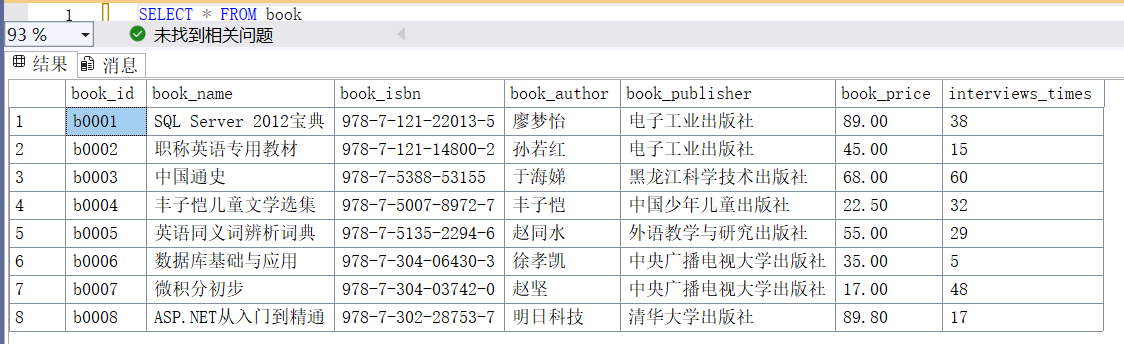
\includegraphics[width=0.8\textwidth]{img/update_result.png}
\caption{更新图书表借阅次数结果}
\label{fig:update}
\end{figure}

\subsubsection{2. 创建借阅次数大于25次的图书信息视图}

\begin{lstlisting}[language=SQL, caption=创建借阅次数大于25次的图书视图]
CREATE VIEW view_popular_books AS
SELECT * FROM book
WHERE interviews_times > 25;
\end{lstlisting}

查询视图结果：
\begin{lstlisting}[language=SQL, caption=查询借阅次数大于25次的图书视图]
SELECT * FROM view_popular_books;
\end{lstlisting}

\begin{figure}[H]
\centering
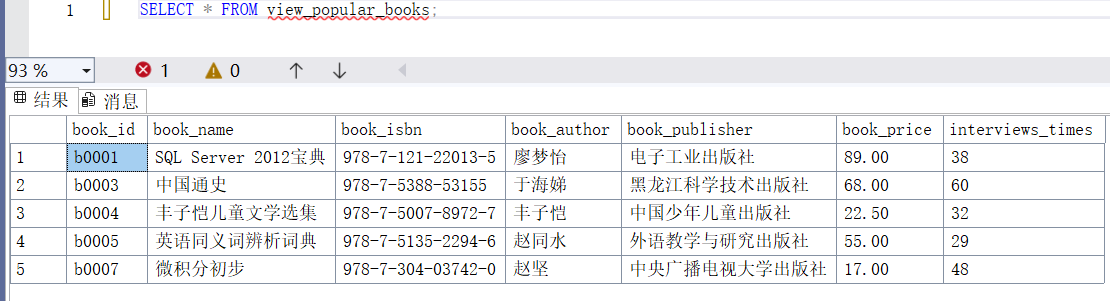
\includegraphics[width=0.8\textwidth]{img/view1_result.png}
\caption{借阅次数大于25次的图书视图查询结果}
\label{fig:view1_result}
\end{figure}

\subsubsection{3. 创建借阅了图书的读者及图书名称视图}

\begin{lstlisting}[language=SQL, caption=创建读者借阅图书信息视图]
CREATE VIEW view_reader_books AS
SELECT r.reader_name, b.book_name
FROM reader r
INNER JOIN record rec ON r.reader_id = rec.reader_id
INNER JOIN book b ON rec.book_id = b.book_id;
\end{lstlisting}

查询视图结果：

\begin{lstlisting}[language=SQL, caption=查询读者借阅图书信息视图]
SELECT * FROM view_reader_books;
\end{lstlisting}

\begin{figure}[H]
\centering
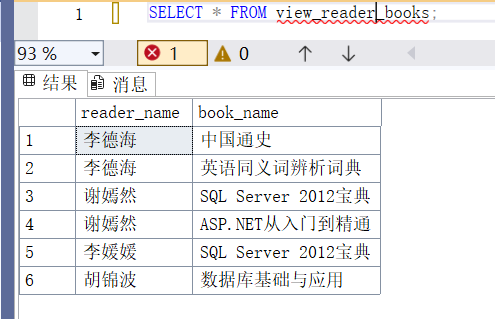
\includegraphics[width=0.8\textwidth]{img/view2_result.png}
\caption{读者借阅图书信息视图查询结果}
\label{fig:view2_result}
\end{figure}

\subsubsection{4. 创建借阅次数大于35次的图书视图（带别名）}

\begin{lstlisting}[language=SQL, caption=创建借阅次数大于35次的图书视图（带别名）]
CREATE VIEW view_highly_popular_books AS
SELECT book_name AS BOOKNAME, interviews_times AS TIMES
FROM book
WHERE interviews_times > 35;
\end{lstlisting}

查询视图结果：

\begin{lstlisting}[language=SQL, caption=查询借阅次数大于35次的图书视图]
SELECT * FROM view_highly_popular_books;
\end{lstlisting}

\begin{figure}[H]
\centering
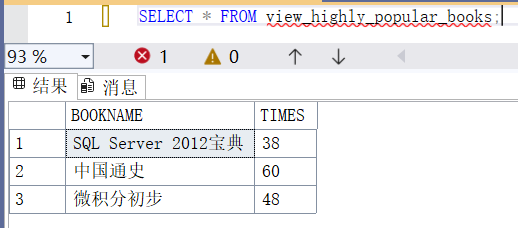
\includegraphics[width=0.8\textwidth]{img/view3_result.png}
\caption{借阅次数大于35次的图书视图查询结果}
\label{fig:view3_result}
\end{figure}

\subsubsection{5. 创建带With Check Option的视图}

\begin{lstlisting}[language=SQL, caption=创建中央广播电视大学出版社图书视图]
CREATE VIEW view_crtvu_books AS
SELECT * FROM book
WHERE book_publisher = '中央广播电视大学出版社'
WITH CHECK OPTION;
\end{lstlisting}

验证With Check Option功能：

尝试通过视图插入中央广播电视大学出版社的图书(应该成功)：

\begin{lstlisting}[language=SQL, caption=通过视图插入符合条件的记录]
INSERT INTO view_crtvu_books 
VALUES ('b0009', '高等数学', '978-7-304-12345-6', '张三', '中央广播电视大学出版社', 10, 28.00);
\end{lstlisting}

\begin{figure}[H]
\centering
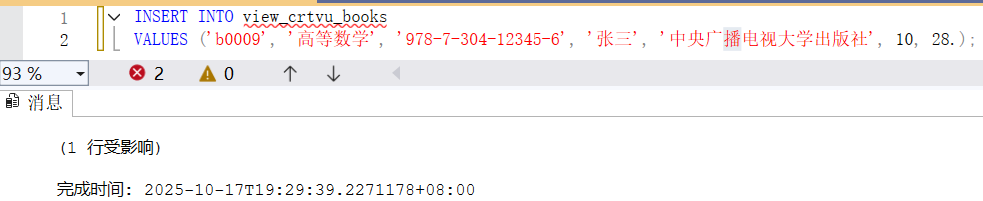
\includegraphics[width=0.8\textwidth]{img/view4_insert_success1.png}
\caption{通过视图插入符合条件的记录（成功）}
\label{fig:view4_insert_success1}
\end{figure}
\begin{figure}[H]
\centering
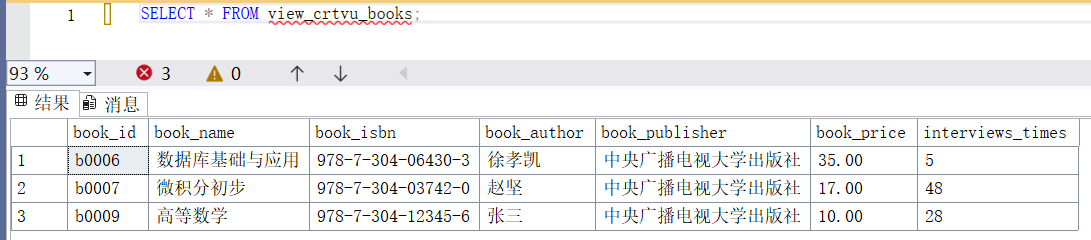
\includegraphics[width=0.8\textwidth]{img/view4_insert_success2.png}
\caption{通过视图插入符合条件的记录（成功）}
\label{fig:view4_insert_success2}
\end{figure}

尝试通过视图插入清华大学出版社的图书（应该失败）：

\begin{lstlisting}[language=SQL, caption=通过视图插入不符合条件的记录]
INSERT INTO view_crtvu_books 
VALUES ('b0010', '数据结构', '978-7-302-12345-6', '李四', '清华大学出版社', 15, 45.00);
\end{lstlisting}

\begin{figure}[H]
\centering
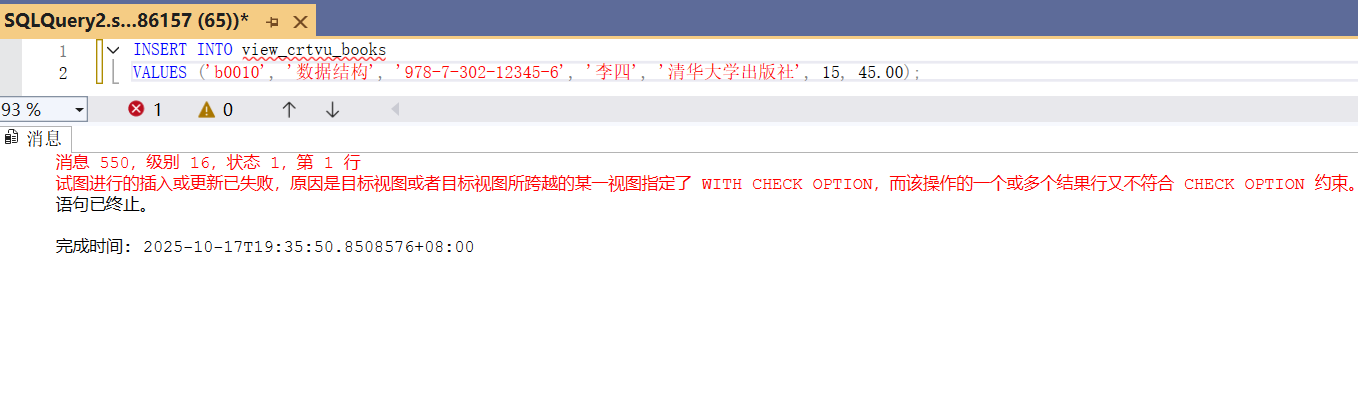
\includegraphics[width=0.8\textwidth]{img/view4_insert_fail.png}
\caption{通过视图插入不符合条件的记录（失败）}
\label{fig:view4_insert_fail}
\end{figure}

% 插入部分已写，补充删除和修改部分

删除一条中央广播电视大学出版社的图书记录（应成功，但实际因外键约束失败）
\begin{lstlisting}[language=SQL, caption=通过视图删除中央广播电视大学出版社的记录]
DELETE FROM view_crtvu_books WHERE book_id = 'b0006';
\end{lstlisting}

\begin{figure}[H]
\centering
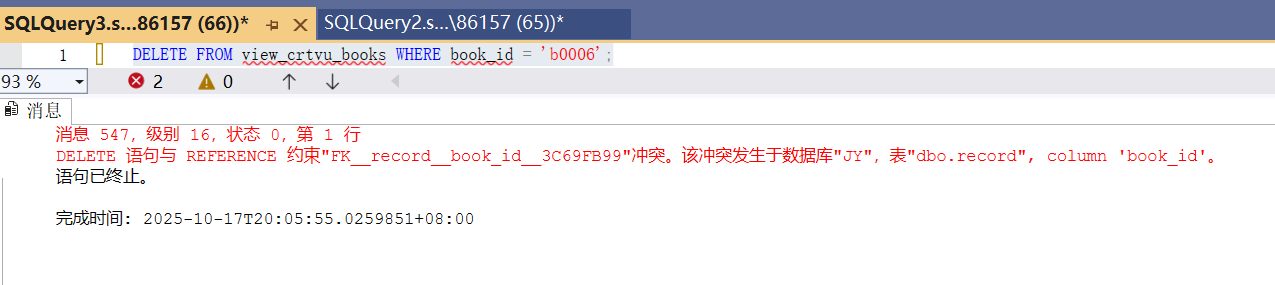
\includegraphics[width=0.8\textwidth]{img/view4_delete.png}
\caption{尝试通过视图删除中央广播电视大学出版社的记录}
\label{fig:view4_delete_success}
\end{figure}

\textbf{说明：}  
实际执行时，因数据库存在外键约束（如 \texttt{record} 表的 \texttt{book\_id} 字段引用 \texttt{book} 表），如果该图书在借阅记录表中被引用，则无法直接删除该图书记录。  

% 修改一条中央广播电视大学出版社的图书记录（应成功）
\begin{lstlisting}[language=SQL, caption=通过视图修改中央广播电视大学出版社的记录]
UPDATE view_crtvu_books SET book_price = 40.00 WHERE book_id = 'b0007';
\end{lstlisting}

\begin{figure}[H]
\centering
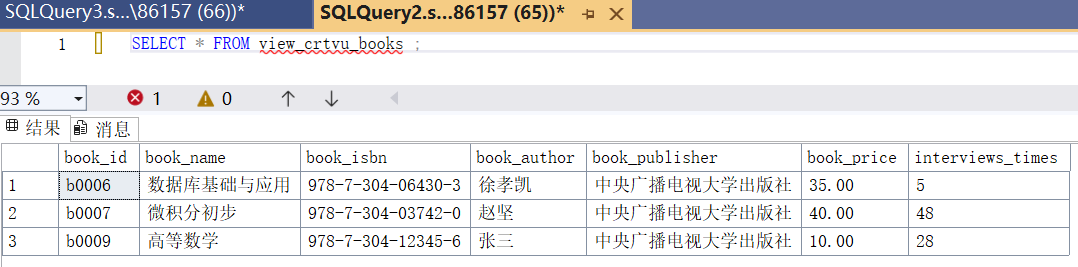
\includegraphics[width=0.8\textwidth]{img/view4_update.png}
\caption{通过视图修改中央广播电视大学出版社的记录（成功）}
\label{fig:view4_update_success}
\end{figure}

\textbf{说明：}  
由于视图 view\_crtvu\_books 只包含“中央广播电视大学出版社”的图书，视图中本身就没有清华大学出版社的记录，因此 DELETE 和 UPDATE 语句不会删除或者更新任何数据，也不会报错。这正体现了 With Check Option 的作用：只能操作视图定义范围内的数据，视图外的数据无法被操作。

\subsubsection{6. 验证视图的可更新性}

测试第一个视图的更新操作：

\begin{lstlisting}[language=SQL, caption=测试第一个视图的更新操作]
UPDATE view_popular_books 
SET book_price = 90.00 
WHERE book_id = 'b0001';
\end{lstlisting}

更新后查询视图内容：

\begin{lstlisting}[language=SQL, caption=查询view\_popular\_books更新后的内容]
SELECT * FROM view_popular_books WHERE book_id = 'b0001';
\end{lstlisting}

\begin{figure}[H]
\centering
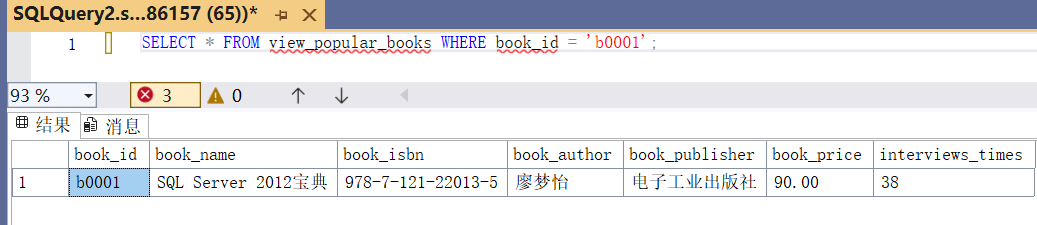
\includegraphics[width=0.8\textwidth]{img/view5_update1.png}
\caption{第一个视图更新操作结果}
\label{fig:view5_update1}
\end{figure}

测试第二个视图的更新操作：

\begin{lstlisting}[language=SQL, caption=测试第二个视图的更新操作]
UPDATE view_reader_books 
SET reader_name = '李德海2' 
WHERE reader_name = '李德海';
\end{lstlisting}

更新后查询视图内容：

\begin{lstlisting}[language=SQL, caption=查询view\_reader\_books更新后的内容]
SELECT * FROM view_reader_books WHERE reader_name = '李德海2';
\end{lstlisting}

\begin{figure}[H]
\centering
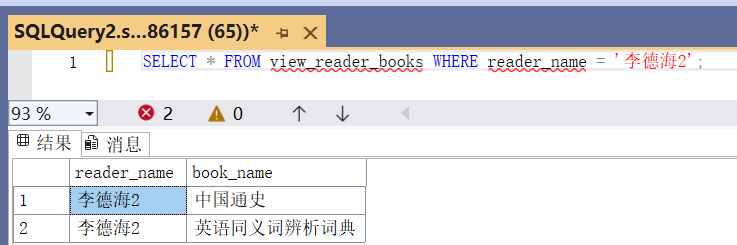
\includegraphics[width=0.8\textwidth]{img/view5_update2.png}
\caption{第二个视图更新操作结果}
\label{fig:view5_update2}
\end{figure}

\subsubsection{7. 删除创建的视图}

\begin{lstlisting}[language=SQL, caption=删除创建的视图]
DROP VIEW view_popular_books;
DROP VIEW view_reader_books;
DROP VIEW view_highly_popular_books;
DROP VIEW view_crtvu_books;
\end{lstlisting}

\begin{figure}[H]
\centering
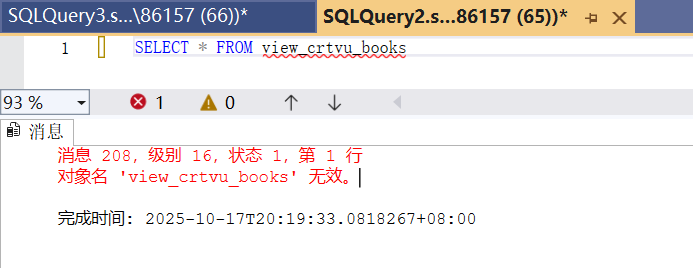
\includegraphics[width=0.8\textwidth]{img/drop_views.png}
\caption{删除视图操作结果}
\label{fig:drop_views}
\end{figure}

\subsection{数据控制}

\subsubsection{1. 创建用户}

\begin{lstlisting}[language=SQL, caption=创建三个用户]
CREATE LOGIN USER1 WITH PASSWORD = 'password1';
CREATE USER USER1 FOR LOGIN USER1;

CREATE LOGIN USER2 WITH PASSWORD = 'password2';
CREATE USER USER2 FOR LOGIN USER2;

CREATE LOGIN USER3 WITH PASSWORD = 'password3';
CREATE USER USER3 FOR LOGIN USER3;
\end{lstlisting}

查询用户是否创建成功
\begin{lstlisting}[language=SQL, caption=查询已创建的用户]
SELECT name FROM sys.database_principals WHERE type = 'S' AND name LIKE 'USER%';
\end{lstlisting}

\begin{figure}[H]
\centering
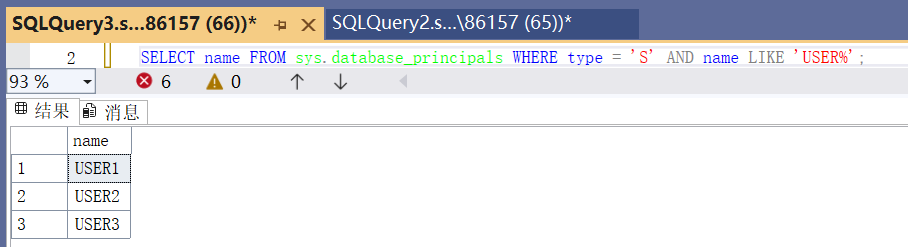
\includegraphics[width=0.8\textwidth]{img/create_users.png}
\caption{创建用户结果}
\label{fig:create_users}
\end{figure}

\begin{figure}[H]
\centering
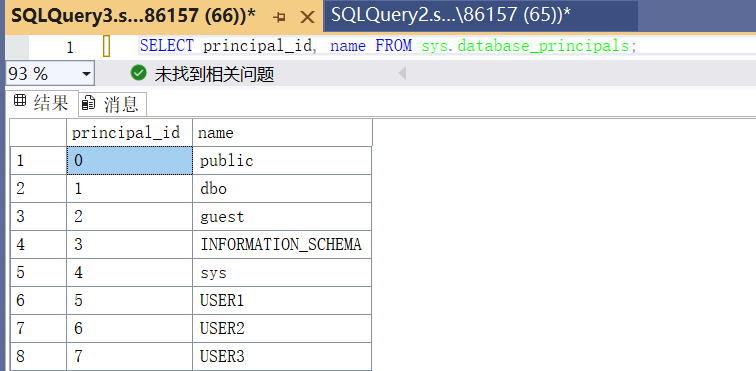
\includegraphics[width=0.8\textwidth]{img/user_id.png}
\caption{查询用户ID对应的结果}
\label{fig:grant1}
\end{figure}

\subsubsection{2. 授予所有用户对图书表的查询权限}

\begin{lstlisting}[language=SQL, caption=授予所有用户对图书表的查询权限]
GRANT SELECT ON book TO USER1, USER2, USER3;
\end{lstlisting}

查询权限授予情况
\begin{lstlisting}[language=SQL, caption=查询用户对book表的权限，id对应见上图]
SELECT grantee_principal_id, permission_name
FROM sys.database_permissions
WHERE major_id = OBJECT_ID('book') AND permission_name = 'SELECT';
\end{lstlisting}

\begin{figure}[H]
\centering
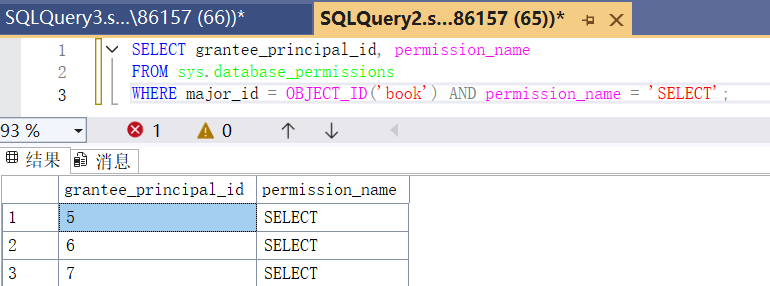
\includegraphics[width=0.8\textwidth]{img/grant1.png}
\caption{授予所有用户对图书表的查询权限}
\label{fig:grant1}
\end{figure}

\subsubsection{3. 授予USER1对读者表的查询、更新权限}

\begin{lstlisting}[language=SQL, caption=授予USER1对读者表的查询、更新权限，并允许传播]
GRANT SELECT, UPDATE ON reader TO USER1 WITH GRANT OPTION;
\end{lstlisting}

\textbf{验证传播权限：}

USER1可以将自己拥有的权限再授予其他用户（如USER2），例如：

\begin{lstlisting}[language=SQL, caption=USER1将SELECT权限授予USER2]
-- 切换到USER1身份执行
EXECUTE AS USER = 'USER1';
GRANT SELECT ON reader TO USER2 WITH GRANT OPTION;
REVERT;
\end{lstlisting}

\begin{lstlisting}[language=SQL, caption=切换到USER2身份验证权限]
EXECUTE AS USER = 'USER2';
SELECT * FROM reader;
REVERT;
\end{lstlisting}

\begin{figure}[H]
\centering
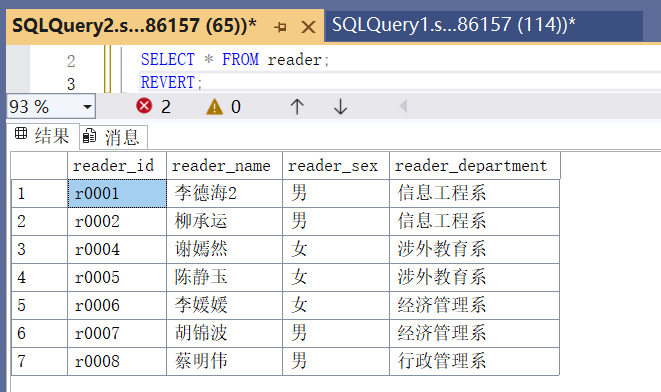
\includegraphics[width=0.8\textwidth]{img/grant2_propagate.png}
\caption{USER1将权限传播给USER2并验证}
\label{fig:grant2_propagate}
\end{figure}

\textbf{说明：}  
在 SQL Server 中，可以使用 `EXECUTE AS USER = 'USER2';` 来模拟以 USER2 身份执行后续语句，`REVERT;` 用于恢复原身份。这样可以验证USER2是否真正获得了查询权限。

\subsubsection{4. 授予USER2对图书表的查询、更新book\_price权限}

\begin{lstlisting}[language=SQL, caption=授予USER2对图书表的查询、更新book\_price权限，并允许传播]
GRANT SELECT, UPDATE(book_price) ON book TO USER2 WITH GRANT OPTION;
\end{lstlisting}

\textbf{验证传播权限：}

USER2可以将自己拥有的权限再授予其他用户（如USER3），例如：

\begin{lstlisting}[language=SQL, caption=USER2将SELECT权限授予USER3]
-- 切换到USER2身份执行
EXECUTE AS USER = 'USER2';
GRANT SELECT ON book TO USER3;
REVERT;
\end{lstlisting}

\begin{lstlisting}[language=SQL, caption=USER3验证是否有SELECT权限]
-- 切换到USER3身份执行
EXECUTE AS USER = 'USER3';
SELECT * FROM book;
REVERT;
\end{lstlisting}

\begin{figure}[H]
\centering
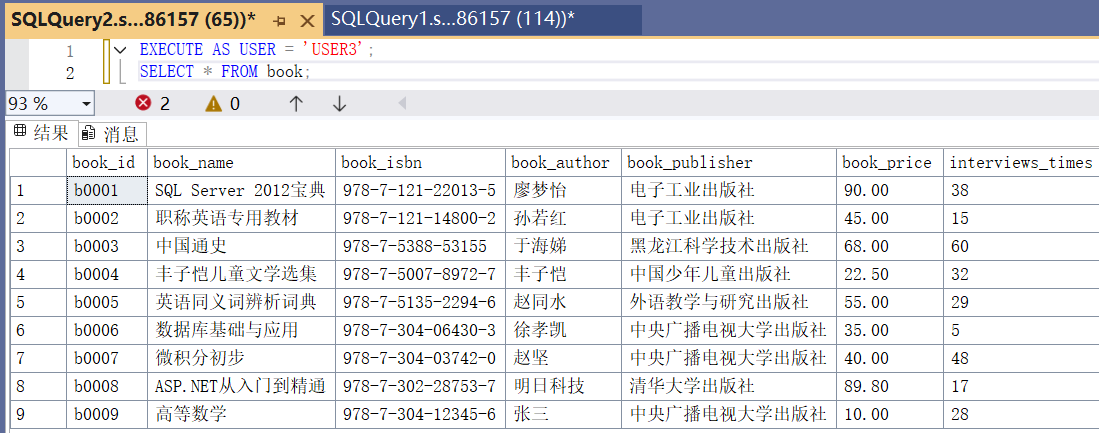
\includegraphics[width=0.8\textwidth]{img/grant3_propagate.png}
\caption{USER2将权限传播给USER3并验证}
\label{fig:grant3_propagate}
\end{figure}

\subsubsection{5. 用户间权限传播}

USER1授予USER2对读者表的查询权限：

\begin{lstlisting}[language=SQL, caption=USER1授予USER2对读者表的查询权限]
-- 切换到USER1身份执行
EXECUTE AS USER = 'USER1';
GRANT SELECT ON reader TO USER2 WITH GRANT OPTION;
REVERT;
\end{lstlisting}

查询USER2对reader表的权限
\begin{lstlisting}[language=SQL, caption=查询USER2对reader表的权限]
EXECUTE AS USER = 'USER2';
SELECT * FROM reader;
REVERT;
\end{lstlisting}

\begin{figure}[H]
\centering
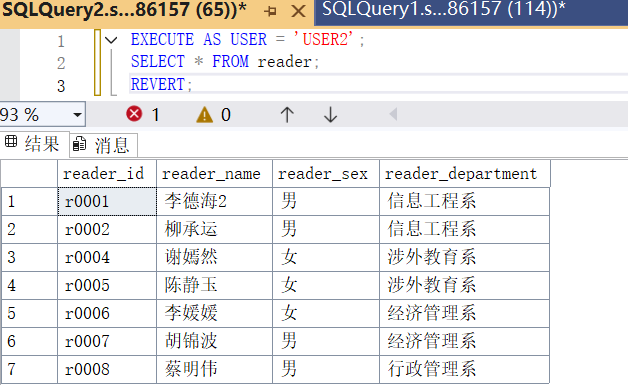
\includegraphics[width=0.8\textwidth]{img/grant4_1.png}
\caption{USER1授予USER2对读者表的查询权限}
\label{fig:grant4_1}
\end{figure}

USER2授予USER3对读者表、图书表的查询权限：

\begin{lstlisting}[language=SQL, caption=USER2授予USER3对读者表、图书表的查询权限]
-- 切换到USER2身份执行
EXECUTE AS USER = 'USER2';
GRANT SELECT ON reader TO USER3;
GRANT SELECT ON book TO USER3;
REVERT;
\end{lstlisting}

查询USER3对reader和book表的权限
\begin{lstlisting}[language=SQL, caption=查询USER3对reader和book表的权限]
EXECUTE AS USER = 'USER3';
SELECT * FROM reader;
SELECT * FROM book;
REVERT;
\end{lstlisting}

\begin{figure}[H]
\centering
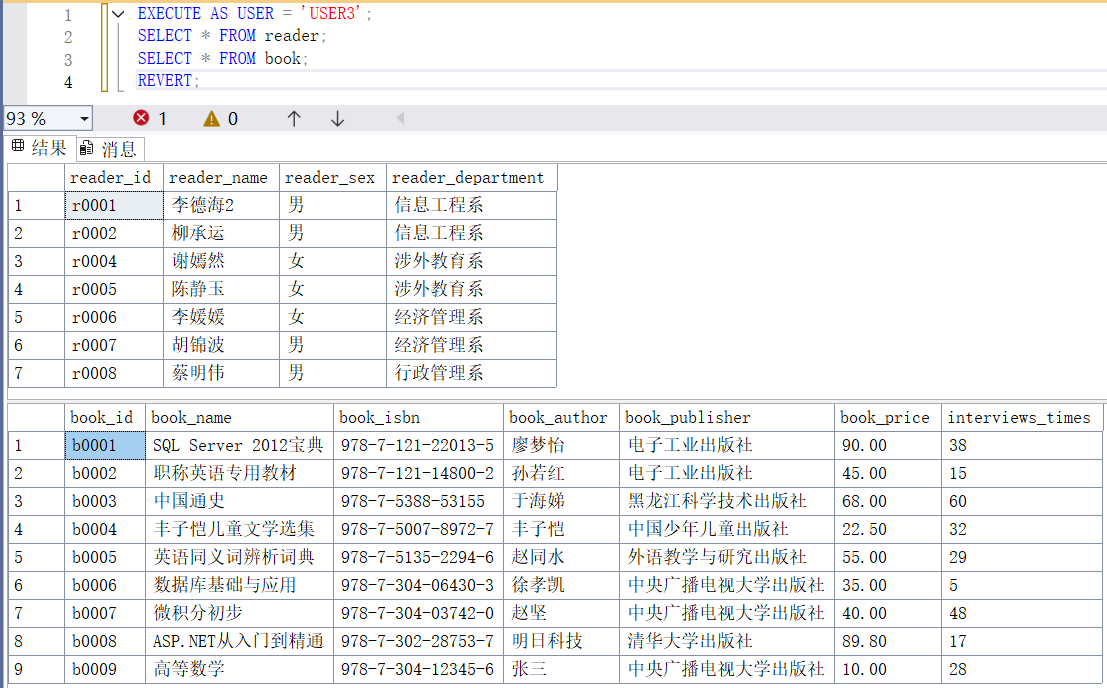
\includegraphics[width=0.8\textwidth]{img/grant4_2.png}
\caption{USER2授予USER3对读者表、图书表的查询权限}
\label{fig:grant4_2}
\end{figure}

\subsubsection{6. 取消权限并验证级联效果}

取消USER1对读者表的查询、更新权限：

\begin{lstlisting}[language=SQL, caption=取消USER1对读者表的权限]
REVOKE SELECT, UPDATE ON reader FROM USER1 CASCADE;
\end{lstlisting}

USER2尝试查询读者表
\begin{lstlisting}[language=SQL, caption=USER2尝试查询读者表]
-- 切换到USER2身份执行
EXECUTE AS USER = 'USER2';
SELECT * FROM reader;
REVERT;
\end{lstlisting}

\begin{figure}[H]
\centering
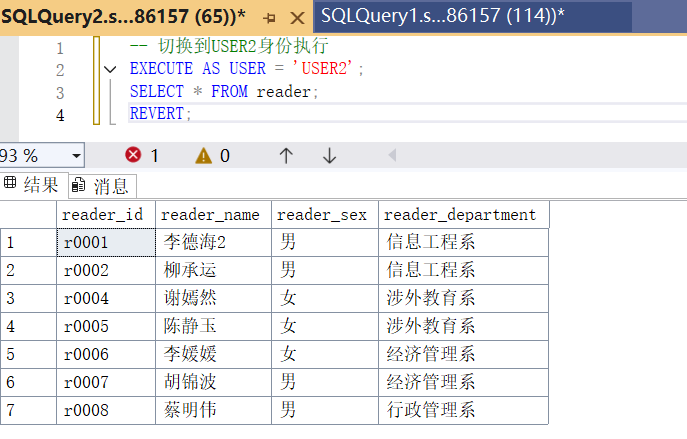
\includegraphics[width=0.8\textwidth]{img/user2_test.png}
\caption{USER2查询读者表测试结果}
\label{fig:user2_query_test}
\end{figure}

验证USER3是否仍能查询reader表和book表：

\begin{lstlisting}[language=SQL, caption=USER3尝试查询reader表和book表]
-- 切换到USER3身份执行
EXECUTE AS USER = 'USER3';
SELECT * FROM reader;
SELECT * FROM book;
REVERT;
\end{lstlisting}

\begin{figure}[H]
\centering
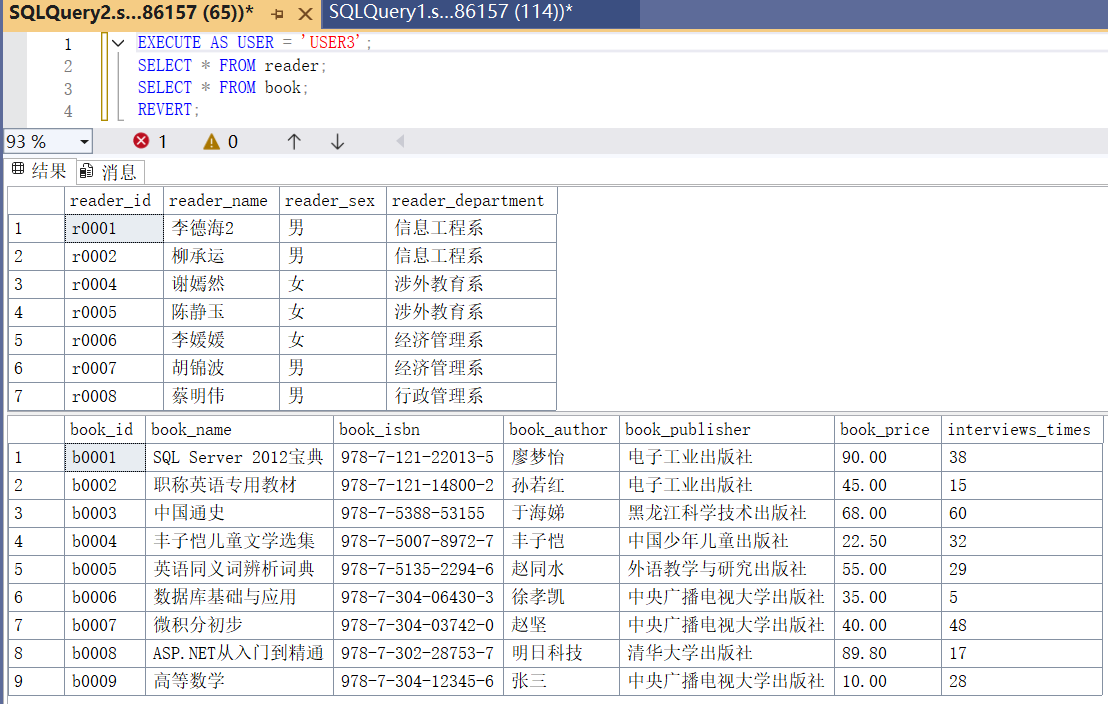
\includegraphics[width=0.8\textwidth]{img/user3_test.png}
\caption{USER3查询表测试结果}
\label{fig:user3_query_test}
\end{figure}

\textbf{结果分析：}

USER2可以成功查询reader表，USER3也可以成功查询reader表和book表。这是因为：

\begin{enumerate}
    \item \textbf{权限传播的独立性}：当USER1将权限授予USER2时，USER2获得的权限是独立的，不依赖于USER1继续拥有该权限。
    \item \textbf{CASCADE的局限性}：虽然使用了CASCADE选项，但它只会撤销直接由USER1授予的权限。如果用户通过其他途径（如管理员直接授予）获得权限，这些权限不会被撤销。
    \item \textbf{多重权限来源}：在实际情况中，USER2可能同时从多个来源获得了对reader表的查询权限（如：步骤2中管理员直接授予的权限，以及步骤3中USER1传播的权限）。
    \item \textbf{权限链的保持}：USER3的权限是由USER2授予的，只要USER2仍有权限且具有传播能力，USER3的权限就会保持有效。
\end{enumerate}

这个实验结果说明了数据库权限管理的复杂性，管理员在进行权限管理时需要谨慎考虑权限的来源和传播路径。

\subsection{总结与思考}

通过本次实验，我全面掌握了数据库视图和权限控制的相关操作：

\paragraph{视图操作总结}
\begin{enumerate}
    \item \textbf{视图创建}：学会了使用CREATE VIEW语句创建各种类型的视图，包括简单视图、连接视图和带列别名的视图。
    \item \textbf{WITH CHECK OPTION}：理解了WITH CHECK OPTION的作用机制，它可以确保通过视图进行的数据修改操作符合视图的定义条件。
    \item \textbf{视图的可更新性}：
       \begin{itemize}
           \item 基于单表的简单视图通常可以更新
           \item 基于多表连接的视图更新会受到限制
           \item 包含聚合函数、GROUP BY等的视图通常不可更新
       \end{itemize}
    \item \textbf{视图管理}：掌握了DROP VIEW语句删除不需要的视图。
\end{enumerate}

\paragraph{权限控制总结}
\begin{enumerate}
    \item \textbf{用户管理}：学会了创建数据库用户的完整流程。
    \item \textbf{权限授予}：掌握了GRANT语句的使用，包括：
       \begin{itemize}
           \item 对象权限（SELECT、UPDATE、INSERT、DELETE）
           \item 列级权限（如UPDATE特定列）
           \item WITH GRANT OPTION子句的使用
       \end{itemize}
    \item \textbf{权限传播}：理解了权限传播机制，拥有GRANT OPTION的用户可以将权限授予其他用户。
    \item \textbf{权限回收}：掌握了REVOKE语句的使用，特别是CASCADE选项的级联回收效果。
\end{enumerate}

\paragraph{关键知识点}
\begin{itemize}
    \item \textbf{权限级联回收}：当使用REVOKE...CASCADE时，由被回收权限的用户授予给其他用户的相同权限也会被回收。
    \item \textbf{视图安全性}：视图可以作为数据访问的安全层，限制用户只能访问特定的数据。
    \item \textbf{权限最小化原则}：在实际应用中应遵循最小权限原则，只授予用户完成工作所必需的最小权限。
\end{itemize}

本次实验加深了我对数据库安全性和数据访问控制的理解，为今后的数据库管理工作奠定了重要基础。

\end{document}